\documentclass[11pt,notitlepage]{article}
\usepackage[utf8]{inputenc}
\usepackage{geometry}                % See geometry.pdf to learn the layout options. There are lots.
\geometry{a4paper}                   % ... or a4paper or a5paper or ... 
%\geometry{landscape}                % Activate for for rotated page geometry
%\usepackage[parfill]{parskip}    % Activate to begin paragraphs with an empty line rather than an indent
\usepackage{graphicx}
\usepackage{amssymb}
\usepackage{epstopdf}
\usepackage{booktabs}     %fancy tables
\usepackage[english]{babel}
\usepackage{ae,aecompl}   % best than T1 fontenc
\usepackage{multicol}
\geometry{reset,
  papersize={210mm,297mm},
  text={170mm,250mm},
  headheight=50pt,
  headsep=10pt,
  hoffset=0cm,
  voffset=0cm,
}

\newcommand{\FIXME}[1]{\marginpar{FIXME}\textsf{FIXME: #1}}

\graphicspath{{schema/pdf/}}

\DeclareGraphicsRule{.tif}{png}{.png}{`convert #1 `dirname #1`/`basename #1 .tif`.png}


\title{Radio Communication Management \\
    {\it ERTMS Subset-026-3.5}}

\author{C{\'e}cile Braunstein\\University of Bremen\\
cecile@informatik.uni-bremen.de}
\date{\today}                                           % Activate to display a given date or no date

\pagestyle{plain}
\begin{document}


\maketitle

% --------------------------------------------------------------------------------------
\begin{abstract}
This document describes the model of the radio communication management The
model has be made from the specification description of the ERTMS subset-026-3.5
baseline 3.
\end{abstract}
The model is composed of two packages : the \emph{system} and the
\emph{requirement}. The system package consists of the SUT model and the TE
model and a set of constants and enumeration types. The
requirement package contains all the requirement and a requirement diagram.
package.
\FIXME{cite SYSML}
% ----------------------------------------------------
\section{Model description}
\label{sec:modeldescription}
The radio communication management module (MoRC) is the user application interacting
with Euroradio protocol. In the following model only the general behaviors is
presented, the actual details of how messages are transported are not relevant
for this description.
\section{Model description}
\label{sec:modeldescription}
The radio communication management module (MoRC) is the user application interacting
with Euroradio protocol. In the following model only the general behaviour is
presented, the actual details of how messages are transported are not relevant
for this description.
% ----------------------------------------------------
\subsection{Interfaces}
\label{subsec:interfaces}


The MoRC is the part of the EVC (European vital computer) responsible for the
management of radio communication.
According to the specification this module interacts directly with the following
on-board modules, as shown in figure \ref{fig:arch}: 
\begin{itemize}
\item (DMI) driver module interface~: receives/displays information from/to the driver,
\item (RTM) radio transmission module~: receives/gives commands from/to the radio
network,
\item (BTM) balise transmission module~: sends transmission request from a balise group,
\item (JRU) Juridical recorder unit~: records part of the data exchange for
\item (OBU tasks) other on-board functions (cf. Subset-026-4.5) used  by the MoRC such as:
\begin{itemize}
\item track conditions managment function  (Subset-026-3.12.1)
for example determine if the ECTS system of the track is compatible with the
system on-board.
\item debug purpose.
\end{itemize}
\end{itemize}

\begin{figure}
\centering
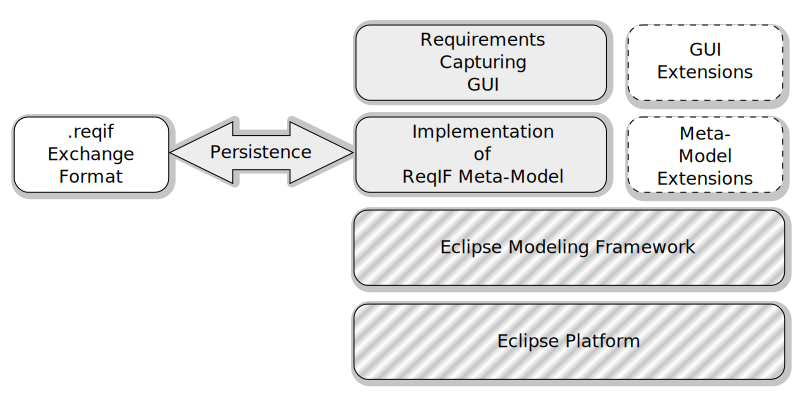
\includegraphics[width =.6\textwidth]{architecture.pdf}
\caption{\label{fig:arch}Interactions of the MoRC and others On-board modules}
\end{figure}

The orders to initiate or terminates a radio communication may come from the
DMI, the BTM, and the RBC (radio block centre) through the RTM. The EVC may also order a radio
communication the subsection \ref{subsec:inputoutput} will give more details.
 on how we have modelled this.
% ----------------------------------------------------
\subsection{Abstraction}
\label{subsec:abstaction}
The MoRC model has been made by direct translation of the specification described
in ERTMS subset-026-3.5 In order to keep the complexity low, some
abstractions have been made. The model's behaviour would be refined in a next step
of the model's design process. In a first step we focus on the communication
protocol between the MoRC and the RTM. This leads us to abstract some behaviours.

First, our representation will not consider the interfaces with the JRU
since it only recorded existing signals and is not relevant for tests
generation
Secondly, the orders coming from BTM, DMI, EVC will be abstracted as only one message
from the on-board. This message will indicate that a communication session
should be started or be ended. We will not distinguished between the different
events that may occured since they follow the same connection protocol. Moreover the discrimination
between these events is not well defined in the specification, we will assume
that the decision is taken by another task of the EVC and that the MoRC task only
 starts or terminates a radio communication
Finaly, the output messages from MoRC to DMI are not considered for the first version.


% ----------------------------------------------------
\subsection{Inputs and outputs messages}
\label{subsec:inputoutput}

Figure \ref{fig:interfaces} shows the messages exchanged at the interface of
the radio communication managment module. The numbers in brackets represent the maximal value the message
may have. Note that in a first version the communication will only be set up
with an RBC, communication with a RIU (radio in-fill unit) are not taken
into account.

\begin{figure}[htpb]
\centering
\includegraphics[width =.6\textwidth]{interface.pdf}
\caption{\label{fig:interfaces} Radio control manager interfaces.}
\end{figure}

\subsubsection{RTM interface}
\verb+MessageOut+, \verb+MessageIn+ are the Euroradio messages, their
possible values are defined in the subset-026-8.4 and the subset-026-7.4. The
test cases define by the subset-076 are performed by analysing the recording of
these messages. In our model we have consider only the relevant messages.
Furthermore, messages are decomposed in variable and packets, these are not
taken into account by our modeling. Our model considers messages only as a number corresponding to an action. 
Table \ref{table:Messages} summarizes the considered messages, the message name
are those used in the model, Id and Packets are those defined in Subset-026-7
and Subset-026-8.

\begin{table}[htbp]
  \begin{tabular}{lclp{.4\textwidth}}\hline
  Message Name & Id & Packets& Description \\\hline
  \verb+TERM_SESSION_TRACK+& 24 & Packet 42 ; Q\_RBC = 0& The RBC orders the EVC to {\bf terminate} a communication with RBC \\
   \verb+INIT_SESSION_ORDER+ & 24 &Packet 42 ; Q\_RBC = 0 & 
   The RBC {\bf orders the initiation} of a communication \\
  \verb+SYS_VERSION+ & 32 & & The RBC {\bf acknowledge the initiation} of a
  communication and gives its system version \\
  \verb+INIT_SESSION_TRACK+ & 38 & &  The RBC {\bf initiates} a communication \\
  \verb+TERM_ACK+ & 39 & &  The RBC {\bf acknoledge} the termination of a communication \\
  \verb+TRANS_OVER_ORDER+ & 131 & & The RBC orders a {\bf transition over} another RBC \\
  \verb+SYS_NO_COMP+ & 154 &&The EVC {\bf acknowledge the establishment with error}. \\
  \verb+INIT_SESSION+& 155 &&  The EVC {\bf initiates} a communication \\
  \verb+TERM_SESSION+ & 156&&The EVC {\bf terminates} a communication  \\
  \verb+SESSION_ESTABLISHED+ & 159 & & The EVC {\bf acknowledge the establishment} of a communication \\
  \verb+NO_MESSAGE+ & 255 & & No messages are send. \\
  \hline
  \end{tabular}
  \caption{\label{table:Messages} Messages exchange during The Managment of
  Radio Communication}
\end{table}

\begin{description}
\item \verb+NID_Rbc+ identifies the RBC it joins the \verb+NID_RBC+ and
\verb+NID_C+ (Subset026-3).
\item \verb+setUp+,\verb+reqSetUp+,\verb+releaseSetUp+ messages are used for setting
or releasing a safe radio communication.
\item \verb+radioHole+ may have the value \verb+BEGIN+, \verb+INSIDE+,
\verb+END+ or
\verb+NONE+ regarding if the train enters, leaves or is in a announced radioHole 
are compatible.
\end{description}

\subsubsection{Interface with others on board functions}
The different cases to initiate or terminate a communication have been abstract
by a single signal. Since the behavior is the same regardless the different
events, we assume that others tasks of the EVC will activate the signal wen
needed.

\begin{description}
\item \verb+orderOnBoard+ represents the order from the on-board EVC to initiate
or terminate a communication. The possible values are the following ones~: 
  \begin{itemize}
  \item \verb+NONE+:  no order;
  \item \verb+INIT+ represents one of these cases :
	\begin{itemize}
	\item Start of mission procedure,
	\item Report a mode change,
	\item Driver change level to 2 or 3,
	\item End of a radio hole,
	\item The balise group orders a radio communication.
	\end{itemize}
  \item \verb+TERM+ represents one of these cases
	\begin{itemize}
	\item End of mission procedure, 
	\item Driver closes the desk,
	\item Error condition detected on-board.
	\item The balise group orders to end up a radio communication.
	\end{itemize}
  \end{itemize}
\item \verb+isCompatible+ is set to 1 if a the track and the on-board systems
(function system version managment)
\end{description}

% ----------------------------------------------------
\subsection{Internal variables}
\label{subsec:internalvar}


The radio management module should take some decision with respect to internal
ERTMS on-board variables. This variable are listed blow. The variable definition
are detailed in subset-026-7.
\begin{itemize}
\item \verb+M_LEVEL+ $\in [0..4]$ represents the levels 0,1,2,3 or STM.
\item \verb+M_ mode+ $\in[0..15]$ represents the on-board operating mode.
\item \verb+safeRadioLink+ $\in \{\mathtt{NOCOM, COM, LOST}\}$ indicates if a safe radio communication is on.
\item \verb+radoComSession+ $\in \{\mathtt{TERMINATED, ESTABLISHED}\}$: indicates if a radio session is established with the track.
\end{itemize} 
Note that the \verb+safeRadioLink+ may be used for the messages given to the
driver.

% ----------------------------------------------------
\subsection{Behaviour}
\label{subsec:behavior}

The behaviour is described figure \ref{fig:behavior}.
A classical transaction starts with an order to established a communication with
an RBC. In this model we assume that the RBC belongs to the RBC accepting list.
Note that we have abstracted the different ways to contact an RBC (last known
number, number entered by the driver ...). Secondly, the MoRC sets up a safe radio
connection, then it initiates a radio communication with the RBC.
An order to terminate a radio communication session may occurred, in this case,
the MoRC sends a termination message to the RBC waits for the acknowledgement and
then releases the safe radio communication.
Our model does not manage the consistency of the successive order, we do not
impose any constraints to when the orders may occur. This may be done by external
tasks.

States \verb+INIT_COM+ and \verb+TERM_COM+ are decomposed as state automata
handling the maximal number of try and the time out of requests.

Sate \verb+COM+ is decomposed as an automaton, it handles the lost of safe
radio.
\begin{figure}[htpb]
\centering
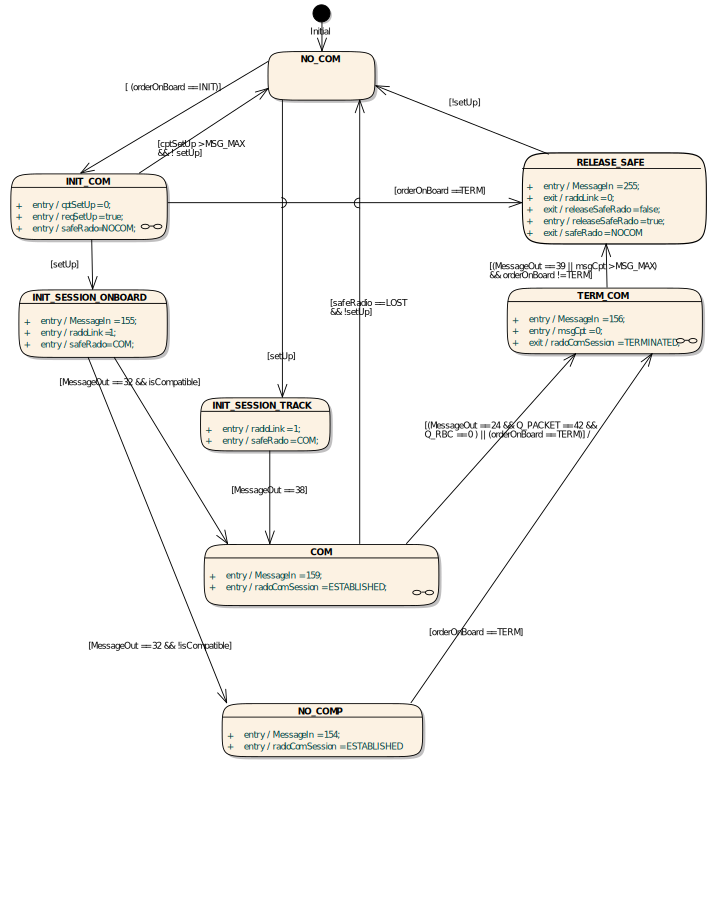
\includegraphics[width=.9\textwidth]{modelRadioManagment-T.pdf}
\caption{\label{fig:behavior}Automata of the radio communication management}
\end{figure}


% ----------------------------------------------------
\section{Requirements Modeling}
\label{sec:requirements}
The model describes in section \ref{sec:modeldescription} is a direct
translation of the SUBSET026-chap 3.5. This section describes how the model is
related to the specification.
SysML offers a modeling constructs to represent text-based requirements and
relationship with other modeling elements. The requirements in EA diagram may be
described in a graphical or tree structured format. The requirement may also
appear directly other diagram. The diagram requirements  intent to  may be imported and
exported from other tools in csv or XMI format.

In this particular experiment, a table document has been made in csv format from
the SRS.
Each requirement is represented as a number that corresponds to the numbers and bullet points
of the specification document. From this list of requirements, one can directly
find the corresponding paragraph in the documents. We had also added the
complete text in a text attribute  for helping the reader. 



The requirement list is then automatically translate to a requirement package  in SysML where
each requirement is a \emph{requirement} SysML element. Our requirement contains
the following attributes :
\begin{itemize}
\item ID : the corresponding name from the SRS
\item Body: the corresponding text from the SRS
\end{itemize}
Figure \ref{fig:req-example} shows an example of the requirement representation.
\begin{figure}[htbp]
\centering
\includegraphics[width=.5\textwidth]{req-example}
\caption{\label{fig:req-example} Example of modeling a requirement}
\end{figure}


Most of requirement refers to the behaviors model as transition of the state-chart
representation.  The link has been made such that each transition satisfy at
least one requirement. Note that in EA, it is not possible to directly link a
transition element to a requirement element, a invariant constraint true has been
added on the transition to make the link.

Others requirement may describe a set of transitions or a more general behavior
property.
In these cases the requirement may be translated as one or more constraints that must be
satisfied by the model. In our model, constraints are invariants expressed in
LTL\cite{PnueliLTL1977}.
SysML does not imposed any language, one can choose other constraints language
such as OCL \cite{ocl2012}.
The following example shows the translation of two requirements into a LTL
properties. The reader should refer to section \ref{sec:deta-model-descr}
for variables and values details.
\begin{description}
\item[REQ-3.5.3.1] "It shall be possible for ERTMS/ETCS on-board equipment and RBC to
initiate a communication session".
\vspace{-1em}
\begin{verbatim}
Finally ((orderOnBoard == 1 || MessageIn == INIT:_SESSION_ORDER || 
MessageIn == INIT_SESSION_TRACK  ) && 
Finally (MessageOut == SESSION_ESTABLISHED))
\end{verbatim}
\end{description}
\begin{description}
\item[REQ-3.5.3.10] "If the establishment of a communication session is
initiated by the RBC, it shall be performed according to the following steps
..."
\vspace{-1em}
\begin{verbatim}
Finally (MessageIn == INIT_SESSION_TRACK && setUp == 1 -> 
Next (MessageOut == SESSION_ESTABLISHED && radioComSession == 1ESTABLISHED)
\end{verbatim}
\end{description}


The requirement diagram only represent the "satisfy" relations between the
requirements and the model. One could refine this diagram and add derive
dependency or containment relationship. Note that in practice we could show the
"satisfy" relations directly on the state-chart view. The separate representation
is more readable. 

% ----------------------------------------------------
\section{Test Generation}
\label{sec:tests}
\subsection{Tool overview}

The RT-Tester test automation tool, made by Verified
\cite{verified_website}, performs automatic test generation, test
execution and real-time test evaluation.  It supports different
testing approach such as unit testing, software integration testing
for component, hardware/software integration testing and system
integration testing.  The RT-Tester version we had used, follows the
model-based testing approach \cite{Peleska2011,rttmbtreport2011} and
it provides the following features :
\begin{itemize}
\item Automated Test Case Generation 
\item Automated Test Data Generation 
\item Automated Test Procedure Generation 
\item Automated Requirement Tracing 
\item Test Management system 
\end{itemize}
Starting from a test model design with UML/SYML, the RT-tester fully
automatically generates test cases. They are then specified as test
data (sequences of stimuli with timing constraints) and used to
stimulate the SUT and run concurently with the generated test
oracles. The test procedure is the combination of the test oracles and
the SUT that can be compiled and executed.

The tool supports test cases/data generation for structural
testing. It automatically generates  reach statement coverage, branch coverage and
modified condition/decision coverage (MC/DC) as far as this is possible.
The test cases may all be linked to requirements ensuring a complete
requirement traceability. 



Finally the tool may produce the documentation of tests for
certification purposes. For each test cases the following document are
produced :
\begin{itemize}
\item {\em Test procedure}: that specifies  how one test case can be
  executed, its associated test data produced and how the SUT
  reactions are evaluated against the expected results.
\item {\em Test report}: that summarizes all relevant information
  about the test execution.
\end{itemize}

In \cite{brauer_efficient_2012}, a general approach  on how to qualify
model-based testing tool according to the standard ISO 26262 ad RTCA
DO178C has been proposed and applied with success to the RT-tester
tool. Following the same  approach compatibility with the CENELEC EN50128
may be easily done. 




\subsection{Test generation}
\begin{itemize}
\item Test coverage
\item Requirement coverage
\item LTL requirement
\end{itemize}
\FIXME{Table coverage summary}
 	


%%% Local Variables: 
%%% mode: latex
%%% TeX-master: "descriptionReport"
%%% End: 


% ----------------------------------------------------
%\section{Others Benchmark}
%Further investigation have been made for modeling other part of the ETCS.
%\include{other_bench}
\bibliographystyle{plain}
\bibliography{model}

\end{document}  
